% Template LaTeX document for CSSR4A Deliverables
% Adapted from documents prepared by EPFL for the RobotCub project
% and subsequently by the University of Skövde for the DREAM project
%
% DV 28/06/2023

\documentclass{CSSRforAfrica}

\usepackage[titletoc,title]{appendix}
\usepackage{latexsym}
\usepackage{comment}
\usepackage{multirow}
\usepackage{subcaption}
\usepackage[breakable,skins,most]{tcolorbox} % Consolidated tcolorbox options
\usepackage{tabularx,colortbl}
\usepackage[tikz]{bclogo} % for boxes
\usepackage{ragged2e}
\usepackage{dirtree}
\usepackage{listings}
\usepackage{textcomp}
\usepackage[colorlinks, urlcolor=blue, linkcolor=black, citecolor=black]{hyperref}
\usepackage{blindtext}
\usepackage[T1]{fontenc}
\usepackage{enumitem}


\lstset{upquote=true}
\renewcommand{\DTstyle}{\footnotesize\sffamily}

%%% for listing ; added by Pam %%%%%%%%%%%%%%%%%%%%%%%%%%%%%%
\captionsetup[figure]{format=hang}
\usepackage{xcolor}
\definecolor{codegreen}{rgb}{0,0.6,0}
\definecolor{codegray}{rgb}{0.5,0.5,0.5}
\definecolor{codepurple}{rgb}{0.58,0,0.82}
\definecolor{backcolour}{rgb}{0.95,0.95,0.92}

\lstdefinestyle{withoutNumbering}{
    backgroundcolor=\color{backcolour},   
    commentstyle=\color{codegreen},
    keywordstyle=\color{magenta},
    stringstyle=\color{codepurple},
    basicstyle=\ttfamily\small,
    breakatwhitespace=false,         
    breaklines=true,                 
    captionpos=b,                    
    keepspaces=true,                 
    showspaces=false,                
    showstringspaces=false,
    showtabs=false,                  
    tabsize=2
}
%%%%%%%%%%%%%%%%%%%%%%%%%%%%%%%%%%%%%%%%%%%%%%%%%%%
\definecolor{backcolour}{rgb}{0.95,0.95,0.95}
\definecolor{irongray}{HTML}{6D6E71}
\definecolor{LightGray}{gray}{0.9}
\definecolor{greenyellow}{rgb}{0.8, 0.7, 0.10} % Example values, adjust as needed

\newcommand{\blank}{~\\}
\newcommand{\checkbox}{{~~~~~~~\leavevmode \put(-7,-1.5){  \huge $\Box$  }}}



\begin{document}
\input{epsf}

%%
%% SHOULD NOT NEED TO BE CHANGED BEFORE THIS POINT
%% ------------------------------------------------
%%

\deliverable{D3.3}                             
\title{D3.3 Software Installation Manual}    

\leadpartner{Carnegie Mellon University Africa}    
\partner{}                                      

\revision{1.13}                          
\deliverabledate{1/10/2023}     
\submissiondate{26/07/2023}   
\revisiondate{21/06/2025}      
\disseminationlevel{PU}
\responsible{ CSSR4Africa Team }   


%%
%% Create the title page
%%
\maketitle

\section*{Executive Summary}
%==============================================================
Deliverable D3.3 is a comprehensive installation manual for the Culturally Sensitive Social Robotics for Africa \href{https://cssr4africa.github.io/}{CSSR4Africa} project. The manual will be continually updated as a living document to ensure it reflects the system's current capabilities. This task aims to document the process of installing and executing the required software components to instantiate the CSSR4Africa system. It provides step-by-step instructions for setting up the development environment and controlling the Pepper robot in both physical and simulated environments.
\label{executive_summary}
\addcontentsline{toc}{section}{Executive Summary}

%\graphicspath{{./figs/}}
\pagebreak
\tableofcontents
\pagebreak


\pagebreak

% \blank
% ~
% \blank
% ADD  subsequent versions here
% \newpage

\section{Introduction}
Software Installation Manual(D3.3) outlines the detailed steps necessary for installing and executing the software critical for deploying parts or the entirety of the CSSR4Africa system, as well as conducting the requisite unit, integration, and system tests. It is designed for systems running a native Ubuntu 20.04 OS and equipped with ROS Noetic. The manual also specifies the NAOqi OS version for the robot as 2.5.10.7.

The manual is divided into several key sections. The initial section, referred to as ``Setting up Pepper Robot, delineates the preliminary configurations required for the Pepper robot before any software installations. Following this, the ``Setting up the Development Environment" section provides comprehensive instructions for preparing the development environments tailored for both the physical robot and the Gazebo simulator. This includes a walkthrough of the prerequisite setup common to both environments, followed by specific installation procedures. Lastly, the ``Installing and Running the CSSR4Africa Software" section discusses installing and initiating the CSSR4Africa software, ensuring a smooth deployment.

\newpage

\section{Setting up Pepper robot}
{\label{setup_pepper}
To configure the Pepper robot for the first time, reference the Pepper Robot Pocket Guide included with your robot when shipped. This guide provides detailed instructions for unboxing and setting up your robot. For additional support, access the online configuration guide at \href{http://doc.aldebaran.com/2-5/family/pepper_user_guide/first_conf_pep.html}{Pepper User Guide}. We are utilizing version 1.8 of the Pepper robot. For comprehensive technical details, including its sensor and actuator capabilities, please refer to the 
\href{http://doc.aldebaran.com/2-5/family/pepper_technical/index_pep.html}{Pepper Technical Detail} \cite{SoftBankDocumentation}. This resource offers a thorough overview of the robot's technical specifications

Next, establish a Wi-Fi connection between the robot and the user's computer. It's advisable to use a dedicated Wi-Fi router for this purpose, rather than relying on a campus wireless network (CMU), to avoid the complications of logging in with a school ID (Andrew ID). To achieve this, connect a router to the campus's network via an Ethernet cable. Upon powering your laptop, instructions on the tablet will guide you to connect to this router. Once connected, the Pepper robot will vocalize its IP address when you press the power button once. This IP address is crucial, as it will be used to establish a connection through ROS (Robot Operating System), enabling communication and control of the robot from your computer. Furthermore, we set up the router for the robot to have a static IP address using the robot's MAC address. 

The MAC address can be found when accessing the Pepper web page as shown in Figure \ref{fig:pepper-web-page}, by opening a web browser and entering the IP address. Then log in by setting the username and password you configured when setting up the robot. Then, using the Wi-Fi MAC address, configure the router to have the Pepper robot's IP address permanently. This can be done by looking at the DHCP or static IP Assignment. Then assign a static IP address by adding a new reservation, entering the MAC  address, and saving the setting. Restart the robot and the router for the changes to take effect.

\begin{figure}[!hbpt]
\centering
\includegraphics[scale=0.30]{images/Pepper-Web-page.png}
\caption{Pepper Web Page}
\label{fig:pepper-web-page}
\end{figure}
}

\section{Setting up the Development Environment}
{
\label{devenv}
This section provides step-by-step instructions for installing a set of software packages required to control the physical Pepper robot and the robot in the Gazebo simulator. Open a new terminal \textit{\textbf{(ctrl + shift + t)}} and type the following commands carefully. 

\subsubsection*{Prerequisite}

{The user needs to have Ubuntu 20.04 running natively for all the software to work properly.} 

\vspace{1em}

\begingroup
\tcbset{%
noteshift/.store in=\mynote@shift,
noteshift=0.2cm
}

\subsection{Method 1: Shell Script Installation}

\begin{enumerate}
\item Ensure Git is installed. If not, install it by running:
\begin{lstlisting}[style=withoutNumbering, language=bash]
sudo apt update
sudo apt install -y git
\end{lstlisting}

\item Create a workspace folder and clone the GitHub repository there:
\begin{lstlisting}[style=withoutNumbering, language=bash]
mkdir -p $HOME/workspace
cd $HOME/workspace
git clone https://github.com/cssr4africa/software-Installation-scripts.git
cd software-Installation-scripts
\end{lstlisting}

\item Make all the shell files executable:
\begin{lstlisting}[style=withoutNumbering, language=bash]
chmod +x *.sh
\end{lstlisting}

\item Run the shell script to install ROS Noetic:
\begin{lstlisting}[style=withoutNumbering, language=bash]
./install_ros_noetic.sh
\end{lstlisting}

\item Run the shell script to install necessary packages and set up the workspace:
\begin{lstlisting}[style=withoutNumbering, language=bash]
./install_pepper_ws.sh
\end{lstlisting}
\end{enumerate}

\hspace{0.9cm}
\begingroup
\tcbset{%
noteshift/.store in=\mynote@shift,
noteshift=0.9cm
}
\begin{tcolorbox}[nobeforeafter,
enhanced,
sharp corners,
toprule=1pt,
bottomrule=1pt,
leftrule=0pt,
rightrule=0pt,
colback=red!20,
left skip=\mynote@shift,
right skip=\mynote@shift,
overlay={\node[left] (mynotenode) at ([xshift=-0.2cm]frame.west) {\textbf{\textcolor{red}{Important:}}} ;},]
There are two alternatives below to set up the development environment for the CSSR4Africa project. If you choose the shell script method (Method 1), the installation ends there, and you can skip the manual installation steps. Only follow Method 2 if you prefer to install ROS Noetic and dependencies manually, step-by-step. 
\end{tcolorbox}
\endgroup
\subsection{Method 2: Manual Installation of Development Environment}
\subsubsection{Installation Steps of the ROS-Noetic }
{

\begin{enumerate}
\item Update and Upgrade the system.
\begin{lstlisting}[style=withoutNumbering, language=bash]
sudo apt update && sudo apt upgrade -y
\end{lstlisting}

\item Install Curl, Git, and Python3-pip.
\begin{lstlisting}[style=withoutNumbering, language=bash]
sudo apt install -y curl git python3-pip net-tools git-lfs
\end{lstlisting}

\item Setup the computer to accept software from \href{http://packages.ros.org}{packages.ros.org.}
\begin{lstlisting}[style=withoutNumbering, language=bash]
sudo sh -c 'echo "deb http://packages.ros.org/ros/ubuntu \
$(lsb_release -sc) main" > /etc/apt/sources.list.d/ros-latest.list'
\end{lstlisting}

\item Setup your keys.
\begin{lstlisting}[style=withoutNumbering, language=bash]
curl -s https://raw.githubusercontent.com/ros/rosdistro/\
master/ros.asc | sudo apt-key add -     
\end{lstlisting}           

\item Update Debian package index.
\begin{lstlisting}[style=withoutNumbering, language=bash]
sudo apt update    
\end{lstlisting}

\item Install ROS Noetic with the default configurations.

\begin{lstlisting}[style=withoutNumbering, language=bash]
sudo apt install ros-noetic-desktop-full
\end{lstlisting}

\item Make ROS environment variables automatically added every time a new shell is launched.
\begin{lstlisting}[style=withoutNumbering, language=bash]
echo "source /opt/ros/noetic/setup.bash" >> $HOME/.bashrc
\end{lstlisting}

\item Sourcing the .bashrc file.
\begin{lstlisting}[style=withoutNumbering, language=bash]
source $HOME/.bashrc
\end{lstlisting}

\item Install additional ROS packages.
\begin{lstlisting}[style=withoutNumbering, language=bash]
sudo apt install -y python3-rosdep python3-rosinstall \
python3-rosinstall-generator python3-wstool build-essential
\end{lstlisting}

\item Initialize rosdep.
\begin{lstlisting}[style=withoutNumbering, language=bash]
sudo rosdep init
rosdep update
\end{lstlisting}
\end{enumerate}
}
\subsubsection{Setting up the Development Environment for the Physical Robot}
\label{phyrob}
\subsubsection*{Installing NAOqi Driver and ROS Packages}

The NAOqi driver is a module that provides bridge capabilities. It publishes sensory data and the pepper position, enabling ROS to call part of the NAOqi API. The driver is dependent on \texttt{naoqi\_libqi, naoqi\_libqicore,} and \texttt{naoqi\_bridge\_msgs} packages. Those packages could be installed using apt-get. The rest of the packages are installed from the source by cloning them from GitHub. The three packages \texttt{naoqi\_dcm\_driver}, \texttt{naoqi\_driver}, and \texttt{pepper\_dcm\_robot} have been modified compared to the official repository on GitHub. Hence, these updated packages are under the CSSR4Africa repository.

\begin{lstlisting}[style=withoutNumbering, language=bash]
# Install the NAOqi driver
sudo apt-get install ros-.*-naoqi-driver

# Create ROS workspace
mkdir -p $HOME/workspace/pepper_rob_ws/src

# Move to the workspace directory
cd $HOME/workspace/pepper_rob_ws/src

# Clone NAOqi DCM driver repository
git clone https://github.com/cssr4africa/naoqi_dcm_driver.git

# Clone NAOqi driver repository
git clone https://github.com/cssr4africa/naoqi_driver.git

# Clone Pepper DCM driver repository
git clone https://github.com/cssr4africa/pepper_dcm_robot.git

# Clone Pepper virtual repository
git clone https://github.com/ros-naoqi/pepper_virtual.git

# Clone the Pepper robot repository
git clone https://github.com/ros-naoqi/pepper_robot.git

# Clone Pepper moveit config repository
git clone https://github.com/ros-naoqi/pepper_moveit_config.git

# Make scripts in naoqi_driver package executable
chmod +x $HOME/workspace/pepper_rob_ws/src/naoqi_driver/scripts/*

# Build the repository
cd .. && catkin_make
# Add the workspace to your ROS environment by sourcing the setup file in the devel folder
source devel/setup.bash

# Add the setup to your .bashrc file so that you don't have to do this every time you open a new terminal
echo "source $HOME/workspace/pepper_rob_ws/devel/setup.bash" >> \
$HOME/.bashrc

# Install additional packages
sudo apt-get install ros-noetic-joint-trajectory-controller
sudo apt-get install ros-noetic-ros-controllers
sudo apt-get install ros-noetic-pepper-meshes

\end{lstlisting}
\subsubsection*{Installing and Configuring the Python NAOqi SDK}
{
The NAOqi Framework, a cross-language programming framework for programming Pepper, supports both C++ and Python. The Python NAOqi SDK was used when the microphone sensor failed to function with the naoqi\_driver, the Python SDK was employed to access the microphone sensors' API. This method allowed the modified naoqi\_driver to publish the captured audio data successfully. Furthermore, since the tablet was not supported by the ROS-NAOqi drivers, the Python SDK was used to provide an interface through ROS. 

\texttt{rospy} is a Python client library for ROS (Robot Operating System), which enables the development of ROS-based applications. It is used mainly to define publishers, subscribers, and services. However, one of the limitations of the Python SDK is that it runs on Python 2, whereas rospy uses Python 3 (ROS-Noetic). To overcome this problem, a UDP socket was used that will send the data from Python 2 to the Python 3 script that receives data and then publishes or provides a ROS service using the rospy.

\begin{enumerate}
\item Change directory to home  
\begin{lstlisting}[style=withoutNumbering, language=bash]
cd $HOME
\end{lstlisting}

\item Installing Python 2.7 
\begin{lstlisting}[style=withoutNumbering, language=bash]
sudo apt install python2

# Check the version of Python
python2 --version
\end{lstlisting}

\item Installing Pip2 
\begin{lstlisting}[style=withoutNumbering, language=bash]
curl https://bootstrap.pypa.io/pip/2.7/get-pip.py --output get-pip.py
\end{lstlisting}

\item Installing the necessary packages

\begin{lstlisting}[style=withoutNumbering, language=bash]
sudo apt-get install libpython2.7
sudo apt-get install libatlas3-base 
sudo python2 get-pip.py
\end{lstlisting}

\item Checking the pip2 version
\begin{lstlisting}[style=withoutNumbering, language=bash]
pip2 --version
\end{lstlisting}

\item Installing NumPy
\begin{lstlisting}[style=withoutNumbering, language=bash]
pip2 install numpy
\end{lstlisting}

\item Download the Python SDK by using the following command. 
\begin{lstlisting}[style=withoutNumbering, language=bash]
wget -S -L https://community-static.aldebaran.com/resources/2.5.5/\
sdk-python/pynaoqi-python2.7-2.5.5.5-linux64.tar.gz
\end{lstlisting}

\item Extract the SDK
\begin{lstlisting}[style=withoutNumbering, language=bash]
tar -xvf pynaoqi-python2.7-2.5.5.5-linux64.tar.gz
\end{lstlisting}

\newpage

\item To ensure that the \texttt{PYTHONPATH} environment variable is automatically set every time a new shell session starts. 

\begin{lstlisting}[style=withoutNumbering, language=bash, escapeinside={(*@}{@*)}]
# If you extracted it in another directory you can set it up by putting the correct path here. 

(*@\color{red}{In addition, write the entire code in one line (avoid using two}@*)
(*@\color{red}{lines)}@*)

echo "export PYTHONPATH=${PYTHONPATH}:$HOME/pynaoqi-python2.7-2.5.5.5-linux64/lib/python2.7/site-packages" >> $HOME/.bashrc
\end{lstlisting}


To apply the changes immediately, you can use the following command 
\begin{lstlisting}[style=withoutNumbering, language=bash]
source $HOME/.bashrc
\end{lstlisting}
\end{enumerate}
}
\subsubsection*{Bring up Pepper}
{
\label{bup}
To establish communication between the computer device and the Pepper robot, the IP address of the computer device, its network interface name, and the IP address of the Pepper robot are needed. To find this information first, ensure the Pepper robot and computer device are on the same network.

\begin{enumerate}
\item \textbf{IP address identification of the computer:}
{
\label{ipsystem}
To find the IP address of the computer device, open a new terminal and execute the \texttt{ifconfig} command.

\begin{figure}[!hbpt]
	\centering
	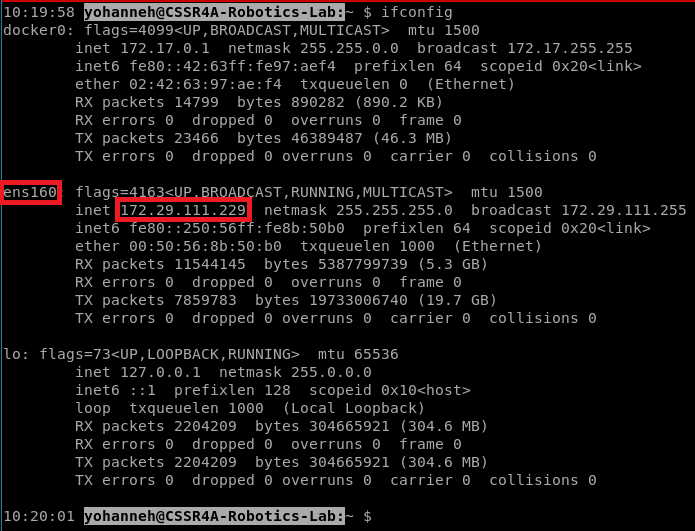
\includegraphics[scale=0.65]{images/Ifconfig.png}
	\caption{\texttt{ifconfig} command output: Network interface name and IP address.}
	\label{fig:ifconfig}
\end{figure}

Upon executing the \texttt{ifconfig} command, the output will display information similar to the illustration shown in Figure \ref{fig:ifconfig}. Please take note of the network interface name and its corresponding IP address as shown in the output. This IP address will be passed as a value for the \texttt{roscore\_ip} argument. Similarly, the network interface must be passed as a value for the \texttt{network\_interface} argument.} 

\item \textbf{IP address identification of the Pepper robot:}
To find the IP address of the Pepper Robot, ensure the robot is powered on and connected to the network. Usually, when the Pepper Robot is booting, it says, ``Hello, I'm Pepper, my internet address is $<robot\_ip >$ (for example, 172.29.111.230)". If you missed it, press the chest button once and take note of that IP address. This IP address will be passed as a value for the robot\_ip argument.

\end{enumerate}
\noindent Using the above IP address of the robot, the IP address, and the network interface name of the computer device, the following instruction will bring Pepper up over ROS, and the NAOqi driver will be launched. Below are the instructions to follow for the sample shown above:

\begin{enumerate}
\item Open a new terminal and bring up the Pepper robot (assuming the robot is turned on).
\begin{lstlisting}[style=withoutNumbering, language=bash]
roslaunch pepper_dcm_bringup pepper_bringup.launch \
robot_ip:=172.29.111.230 roscore_ip:=172.29.111.229 \
network_interface:=ens160
\end{lstlisting}

\item Open a new terminal and launch the NAOqi driver.
\begin{lstlisting}[style=withoutNumbering, language=bash]
roslaunch naoqi_driver naoqi_driver.launch nao_ip:=172.29.111.230 \
roscore_ip:=172.29.111.229 network_interface:=ens160
\end{lstlisting} 
\end{enumerate}
}

\subsubsection{Setting up the Development Environment for the Gazebo Simulator}
\label{simulator}
Section \ref{phyrob} assumes access to a physical Pepper robot. However, circumstances may arise where testing software without the physical robot becomes necessary. In such cases, a simulator can serve as an alternative. This section explains how to control the Pepper robot within a Gazebo simulator. The simulation is based on an open-source Pepper ROS environment developed by Sam Pfeiffer.\footnote{The Pepper ROS simulator is available on the following links: \url{https://github.com/awesomebytes/pepper\_virtual}}. The installation of the Gazebo simulator is presented below.

\subsubsection*{Installation of the Gazebo Simulator}
To set up the Gazebo simulator for the Pepper robot, follow the instructions below.

\begin{enumerate}
\item \textbf{Setup Pepper in the Gazebo Simulator}
\begin{enumerate}
\item Make a separate workspace for the simulator installation.
\begin{lstlisting}[style=withoutNumbering, language=bash]
mkdir -p $HOME/workspace/pepper_sim_ws/src
cd $HOME/workspace/pepper_sim_ws/src
\end{lstlisting} 

\item Clone the necessary packages from the GitHub repository.
\begin{lstlisting}[style=withoutNumbering, language=bash]
git clone -b correct_chain_model_and_gazebo_enabled \
https://github.com/awesomebytes/pepper_robot
\end{lstlisting} 

\begin{lstlisting}[style=withoutNumbering, language=bash]
git clone -b simulation_that_works \
https://github.com/awesomebytes/pepper_virtual
\end{lstlisting} 

\begin{lstlisting}[style=withoutNumbering, language=bash]
git clone https://github.com/cssr4africa/\gazebo_model_velocity_plugin
\end{lstlisting} 

\item Install additional libraries.
\begin{lstlisting}[style=withoutNumbering, language=bash]
sudo apt-get install ros-noetic-tf2-sensor-msgs \
ros-noetic-ros-control ros-noetic-ros-controllers \
ros-noetic-gazebo-ros ros-noetic-gazebo-ros-control \
ros-noetic-gazebo-plugins ros-noetic-controller-manager \
ros-noetic-ddynamic-reconfigure-python
\end{lstlisting}

\item Install Pepper Mesh.
\begin{lstlisting}[style=withoutNumbering, language=bash]
sudo apt-get install ros-noetic-pepper-meshes
\end{lstlisting}

\item Build the packages in the workspace.
\begin{lstlisting}[style=withoutNumbering, language=bash]
cd .. && catkin_make -DSIMULATOR=ON
\end{lstlisting}

\begingroup
\tcbset{%
noteshift/.store in=\mynote@shift,
noteshift=0.2cm
}
\begin{tcolorbox}[nobeforeafter,
enhanced,
sharp corners,
toprule=1pt,
bottomrule=1pt,
leftrule=0pt,
rightrule=0pt,
colback=yellow!20,
left skip=\mynote@shift,
right skip=\mynote@shift,
overlay={\node[left] (mynotenode) at ([xshift=-\mynote@shift]frame.west) {\textbf{\textcolor{greenyellow}{Note:}}} ;},]
After setting up the physical robot's environment, follow step (f) to modify the \texttt{.bashrc} will result in the simulator environment being sourced last, overriding the physical robot's settings. If your main work is with the physical robot, consider skipping this step. You can manually \texttt{source devel/setup.bash} when necessary for simulator tasks to maintain the correct environment setup 
\end{tcolorbox}
\endgroup

\item Make ROS environment variables automatically added every time a new shell is launched.
\begin{lstlisting}[style=withoutNumbering, language=bash]
echo "source $HOME/workspace/pepper_sim_ws/devel/setup.bash" >> \
$HOME/.bashrc
\end{lstlisting}

\begin{lstlisting}[style=withoutNumbering, language=bash]
source $HOME/.bashrc
\end{lstlisting}

\end{enumerate}
\item \textbf{Run the Pepper Gazebo Simulator}
\begin{enumerate}[leftmargin=0pt,labelsep=0.5em]
\item Start the Gazebo simulation.
\begin{lstlisting}[style=withoutNumbering, language=bash]
roslaunch pepper_gazebo_plugin \
pepper_gazebo_plugin_in_office_CPU.launch
\end{lstlisting}

\begin{figure}[!hbpt]
\centering
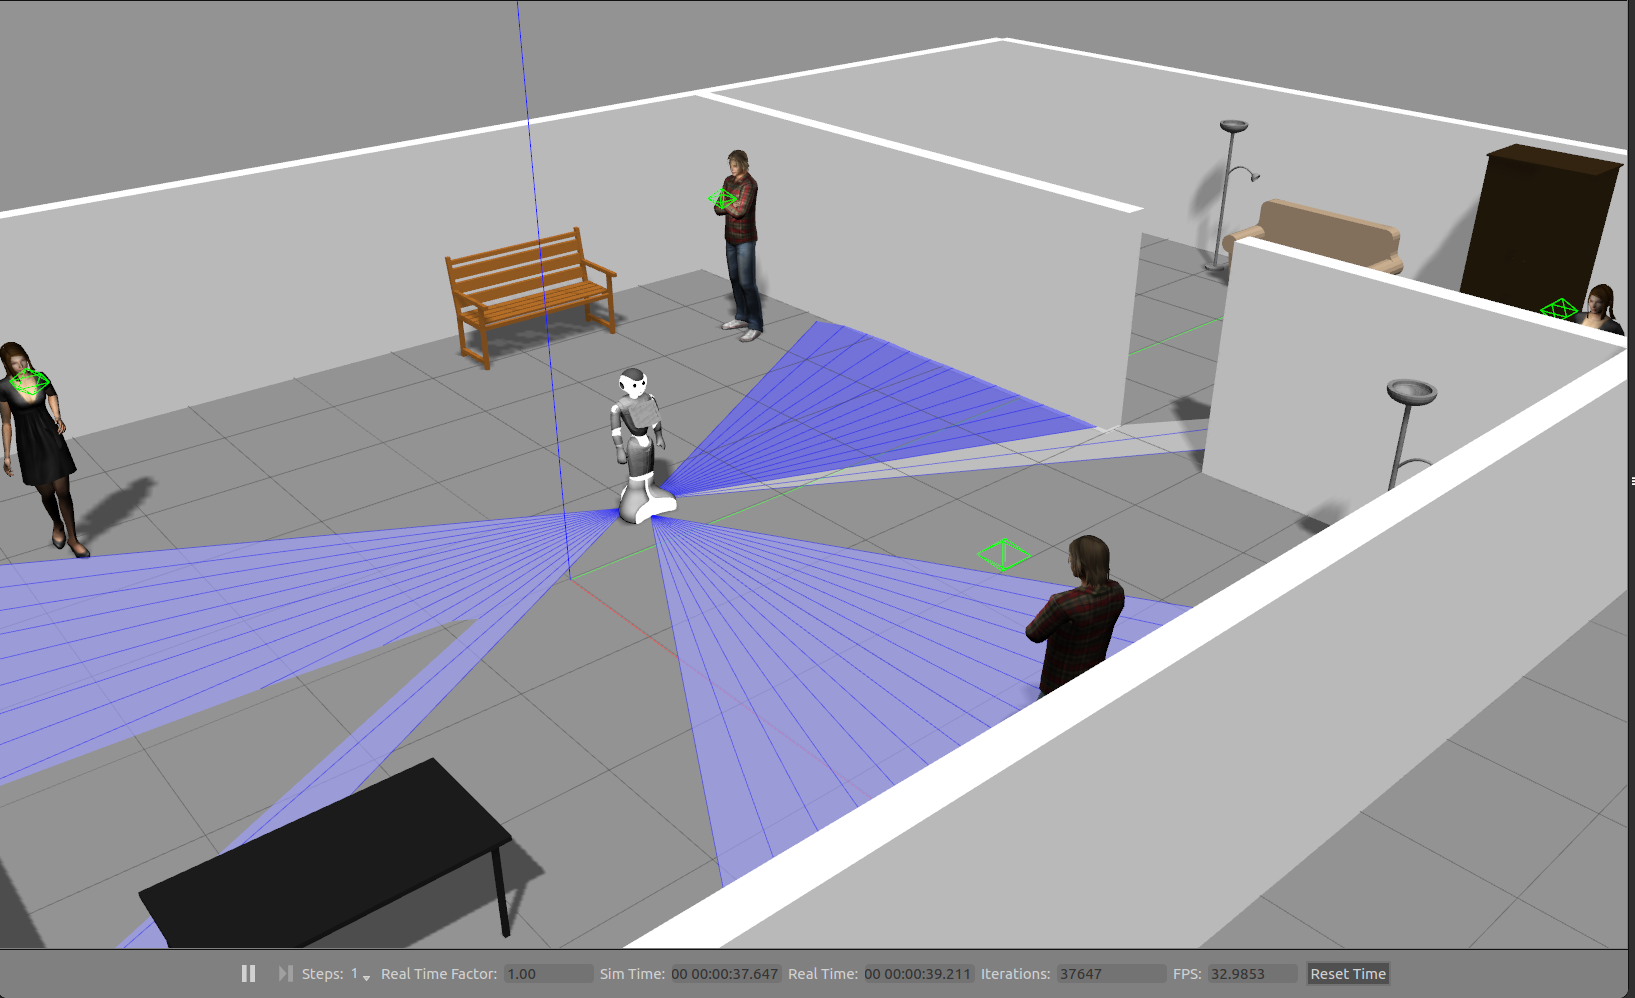
\includegraphics[scale=0.25]{./images/gazebo-screenshot.png}
\caption{Pepper Gazebo simulation environment.}
\label{fig:gazebo-sim}
\end{figure}

\noindent Once you’ve successfully launched the simulator, your environment should match Figure~\ref{fig:gazebo-sim}. To visualize in RViz, open a new terminal and run:

\begin{lstlisting}[style=withoutNumbering, language=bash]
rosrun rviz rviz -d `rospack find pepper_gazebo_plugin`/config/pepper_sensors.rviz
\end{lstlisting}
\end{enumerate}
\end{enumerate}

\newpage
The visualization that appears on RViz after launching will have a similar appearance to Figure \ref{fig:rviz}.

\begin{figure}[!hbpt]
\centering
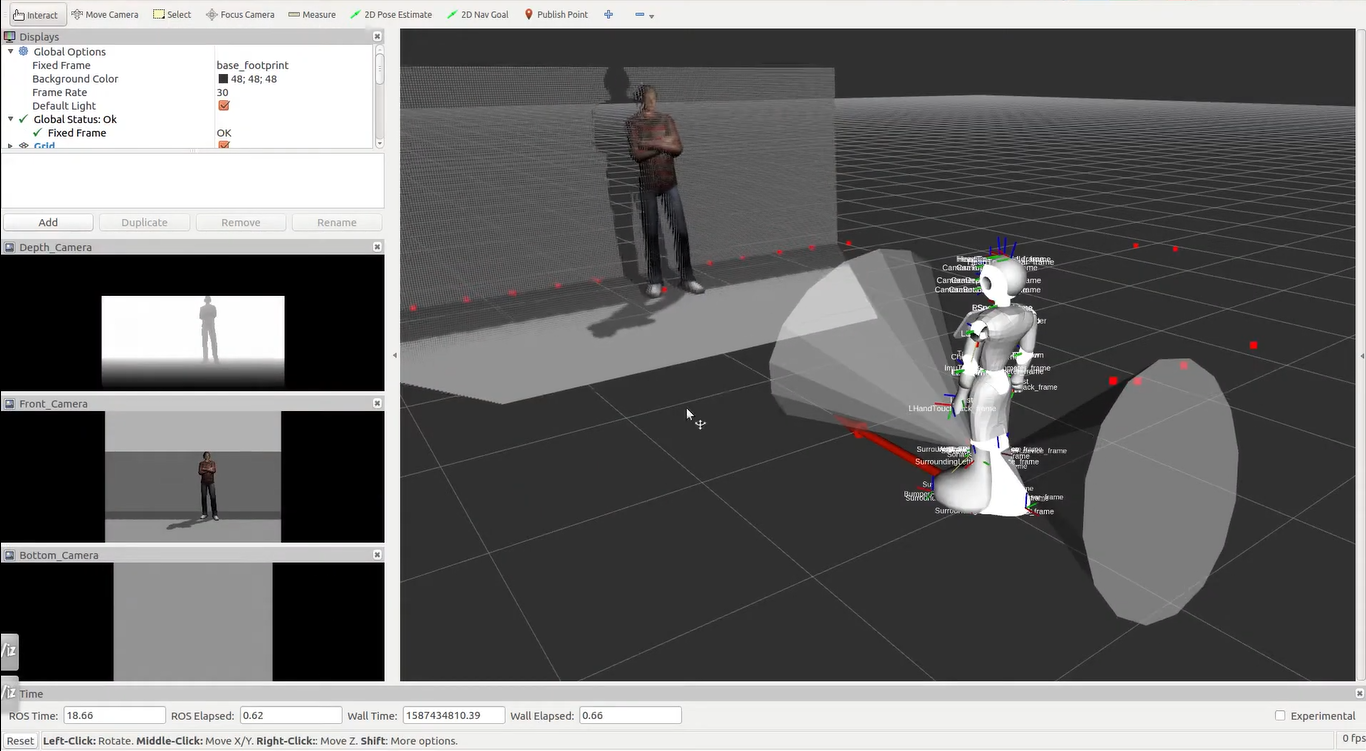
\includegraphics[scale=0.40]{./images/rviz.png}
\caption{Visualization of the simulation on RViz.}
\label{fig:rviz}
\end{figure}



\clearpage
\section{Installing and Running the CSSR4Africa Software}
\label{cssr4africa}

\subsection{Using Shell Script to install CSSR4Africa Software}

\hspace{0.9cm}
\begingroup
\tcbset{%
noteshift/.store in=\mynote@shift,
noteshift=1.2cm
}
\begin{tcolorbox}[nobeforeafter,
enhanced,
sharp corners,
toprule=1pt,
bottomrule=1pt,
leftrule=0pt,
rightrule=0pt,
colback=red!20,
left skip=\mynote@shift,
right skip=\mynote@shift,
overlay={\node[left] (mynotenode) at ([xshift=-0.5cm]frame.west) {\textbf{\textcolor{red}{Important:}}} ;},]
Inside the Software Installation Scripts directory that was cloned in section 3.1, run the following script. This installs all the CSSR4Africa software. Section 4.2 should be skipped if this script runs successfully to completion. 
\end{tcolorbox}
\endgroup

\begin{lstlisting}[style=withoutNumbering, language=bash]
# Change into the Software Installation Scripts directory
cd $HOME/workspace/software-Installation-scripts
\end{lstlisting}

\begin{lstlisting}[style=withoutNumbering, language=bash]
# Execute the installer for the CSSR4Africa package
./install_cssr4africa_package.sh
\end{lstlisting}


\subsection{Manual Installation of the CSSR4Africa Software}
This section will guide you through the installation process of the CSSR4Africa software in the source directory of the workspace. The software installation for the physical and simulator environments will be discussed below.

\subsubsection{Installing the CSSR4Africa Software for the Physical Robot}
The outlined steps for installing the CSSR4Africa software for the physical robot are as follows:
\begin{lstlisting}[style=withoutNumbering, language=bash]
# Move to the source directory of the workspace
cd $HOME/workspace/pepper_rob_ws/src

# Clone the CSSR4Africa software from the GitHub repository
git clone https://github.com/cssr4africa/cssr4africa.git

# Build the source files
cd .. && catkin_make

# Clone the models from HuggingFace
cd && git lfs install
git clone https://huggingface.co/cssr4africa/cssr4africa_models

# Prepare and move the face detection models
mkdir -p "$HOME/workspace/pepper_rob_ws/src/cssr4africa/cssr_system/face_detection/models"
mv cssr4africa_models/face_detection/models/* \
"$HOME/workspace/pepper_rob_ws/src/cssr4africa/cssr_system/face_detection/models/"

# Prepare and move the person detection models
mkdir -p "$HOME/workspace/pepper_rob_ws/src/cssr4africa/cssr_system/person_detection/models"
mv cssr4africa_models/person_detection/models/* \
"$HOME/workspace/pepper_rob_ws/src/cssr4africa/cssr_system/person_detection/models/"

# Clone the unit test data from HuggingFace
cd && git lfs install
git clone https://huggingface.co/cssr4africa/cssr4africa_unit_tests_data_files

# Prepare and move the face detection test data
mkdir -p "$HOME/workspace/pepper_rob_ws/src/cssr4africa/unit_tests/face_detection_test/data"
mv cssr4africa_unit_tests_data_files/face_detection_test/data/* \
"$HOME/workspace/pepper_rob_ws/src/cssr4africa/unit_tests/face_detection_test/data/"

# Prepare and move the person detection test data
mkdir -p "$HOME/workspace/pepper_rob_ws/src/cssr4africa/unit_tests/person_detection_test/data"
mv cssr4africa_unit_tests_data_files/person_detection_test/data/* \
"$HOME/workspace/pepper_rob_ws/src/cssr4africa/unit_tests/person_detection_test/data/"

# Remove the cloned model and test data directories to clean up
rm -rf ~/cssr4africa_models
rm -rf ~/cssr4africa_unit_tests_data_files
\end{lstlisting}

\noindent Upon completing the installation above, the \textbf{src} folder within the development environment's workspace will contain the CSS4Africa software meta-package and all the necessary packages for the project. 

\newpage

As of now, only six software have been uploaded in the \texttt{cssr\_system} and \texttt{unit\_tests} directory: \texttt{animateBehaviour}, \texttt{faceDetection}, \texttt{soundDetection}, \texttt{gestureExecution}, \texttt{overtAttention}, $ $and \texttt{personDetection}. 

Figure \ref{fig:pepper-robot-workspace-directory} shows the directory structure of the workspace for reference.
\begin{figure}[ht]

{\small 
\dirtree{%
.1 workspace.
.2 pepper\_rob\_ws.
.3 build.
.3 devel.
.3 src.
.4 cssr4africa.
.5 cssr\_system.
.6 animateBehavior.
.6 face\_detection.
.6 gestureExecution.
.6 overtAttention.
.6 person\_detection.
.6 sound\_detection.
.5 dashboard.
.5 pepper\_interface\_tests.
.5 system\_tests.
.5 unit\_tests.
.6 animateBehaviourTest.
.6 face\_detection\_test.
.6 gestureExecutionTest.
.6 overtAttentionTest.
.6 person\_detection\_test.
.6 sound\_detection\_test.
.4 naoqi\_dcm\_driver.
.4 naoqi\_driver.
.4 pepper\_dcm\_robot.
.4 pepper\_moveit\_config.
.4 pepper\_robot.
.4 pepper\_virtual.
}
}

\caption{Directory structure for the CSSR4Africa software repository.}
\label{fig:pepper-robot-workspace-directory}
\end{figure}

\subsubsection{Installing the CSSR4Africa Python Virtual Environment}
The CSSR4Africa system requires dedicated Python virtual environments for different components. This section provides step-by-step instructions for setting up these environments.


\subsubsection*{Face and Person Detection Environment}
The face and person detection system requires Python 3.10 with PyTorch and CUDA support.

\newpage
\subsubsection*{System Package Installation}
First, update the system packages and install Python 3.10:
\begin{lstlisting}[style=withoutNumbering, language=bash]
# Update system packages
sudo apt update && sudo apt upgrade -y

# Add the deadsnakes PPA for Python versions
sudo apt install software-properties-common -y
sudo add-apt-repository ppa:deadsnakes/ppa -y
sudo apt update

# Install Python 3.10
sudo apt install python3.10 python3.10-venv python3.10-distutils -y

# Verify Python installation
python3.10 --version
\end{lstlisting}

\subsubsection*{Virtual Environment Setup}
Create and configure the Python virtual environment for face and person detection:
\begin{lstlisting}[style=withoutNumbering, language=bash]
# Create the virtual environment directory
mkdir -p $HOME/workspace/pepper_rob_ws/src/cssr4africa_virtual_envs
cd $HOME/workspace/pepper_rob_ws/src/cssr4africa_virtual_envs

# Create a virtual environment
python3.10 -m venv cssr4africa_face_person_detection_env

# Activate the virtual environment
source cssr4africa_face_person_detection_env/bin/activate

# Upgrade pip in the virtual environment
pip install --upgrade pip
\end{lstlisting}

\subsubsection*{PyTorch and Dependencies Installation}
Install PyTorch with CUDA support and the required dependencies:
\begin{lstlisting}[style=withoutNumbering, language=bash]
# Install PyTorch with CUDA support
pip3 install torch torchvision torchaudio --index-url https://download.pytorch.org/whl/cu118

# Install additional requirements from the project requirements file
pip install -r ~/workspace/pepper_rob_ws/src/cssr4africa/cssr_system/face_detection/face_detection_requirements_x86.txt
\end{lstlisting}

\subsubsection*{Activating the Face and Person Detection Environment}
To use the face and person detection system, activate the environment:
\begin{lstlisting}[style=withoutNumbering, language=bash]
# Navigate to the virtual environment directory
cd $HOME/workspace/pepper_rob_ws/src/cssr4africa_virtual_envs

# Activate the environment
source cssr4africa_face_person_detection_env/bin/activate
\end{lstlisting}

The face and person detection virtual environment setup is now complete.

\subsubsection*{Sound Detection Environment}
The sound detection system requires Python 3.8 with its own set of dependencies.

\subsubsection*{System Package Installation for Sound Detection}
Ensure Python 3.8 virtual environment tools are installed:
\begin{lstlisting}[style=withoutNumbering, language=bash]
# Update system packages (if not already done)
sudo apt update && sudo apt upgrade -y

# Install Python virtual environment tools
sudo apt install python3.8-venv -y
\end{lstlisting}

\subsubsection*{Sound Detection Virtual Environment Setup}
Create and configure the Python virtual environment for sound detection:
\begin{lstlisting}[style=withoutNumbering, language=bash]
# Navigate to the virtual environments directory
cd $HOME/workspace/pepper_rob_ws/src/cssr4africa_virtual_envs/

# Create a virtual environment for sound detection
python3.8 -m venv cssr4africa_sound_detection_env

# Activate the virtual environment
source cssr4africa_sound_detection_env/bin/activate

# Upgrade pip in the virtual environment
pip install --upgrade pip
\end{lstlisting}

\subsubsection*{Sound Detection Dependencies Installation}
Install the required packages for sound detection:
\begin{lstlisting}[style=withoutNumbering, language=bash]
# Install required packages from the requirement file.
pip install -r ~/workspace/pepper_rob_ws/src/cssr4africa/cssr_system/sound_detection/sound_detection_requirements.txt
\end{lstlisting}

\subsubsection*{Activating the Sound Detection Environment}
To use the sound detection system, activate the dedicated environment:
\begin{lstlisting}[style=withoutNumbering, language=bash]
# Navigate to the virtual environment directory
cd $HOME/workspace/pepper_rob_ws/src/cssr4africa_virtual_envs

# Activate the sound detection environment
source cssr4africa_sound_detection_env/bin/activate
\end{lstlisting}

The sound detection virtual environment setup is now complete.

\subsubsection{Installing the CSSR4Africa Software for the Simulator Robot}
\label{sim-soft}
The steps for installing the CSSR4Africa software for the simulated environment will be presented as follows:

\begin{lstlisting}[style=withoutNumbering, language=bash]
# Move to the source directory of the workspace
cd $HOME/workspace/pepper_sim_ws/src

# Clone the CSSR4Africa software from the GitHub repository
git clone https://github.com/cssr4africa/cssr4africa.git
# Build the source files
cd .. && catkin_make -DSIMULATOR=ON
\end{lstlisting}

\subsection{Running the CSSR4Africa Software}
In this section, the execution of the unit, integration, and system tests of the CSSR4Africa software packages will be presented.

\subsubsection{The Pepper Interface Tests Package}
The pepper\_interface\_test package contains the node files that have been written to perform the unit tests to evaluate the functionality and performance of sensors and actuators on the physical robot and the robot simulator. The directory structure of the pepper\_interface\_test is shown in Figure \ref{fig:pepper-interface-tests-directory-structure}.

The actuator test includes testing the head, hand, arm, leg, and wheels. The sensor test comprehensively assesses multiple sensors: front and back sonar, front and bottom cameras, stereo and depth cameras, laser sensor, microphone, odometry, and joint states.

\noindent To run the test on the physical robot, change the first line of the actuatorTestConfiguration.ini and sensorTestConfiguration.ini files to \texttt{platform robot}. On the other hand, to run the test on the simulator platform, change the first line of the actuatorTestConfiguration.ini and sensorTestConfiguration.ini files to \texttt{platform simulator}. 

\noindent Before starting the test on the physical robot, run the launch file of the \texttt{pepper\_interface\_tests} package, either the actuatorTestLaunchRobot.launch or sensorTestLaunchRobot.launch. Please replace the variables \texttt{robot\_ip, roscore\_ip,} and \texttt{network\_interface\_name} with the values obtained from the section \ref{bup}. Then, proceed to run the actuator and sensor test.\\

\begin{lstlisting}[style=withoutNumbering, language=bash]
cd $HOME/workspace/pepper_rob_ws
source devel/setup.bash
\end{lstlisting}

\noindent Before starting the test on the robot, open a new terminal and launch either the sensor launch file or the actuator launch file.\\

\begingroup
\tcbset{%
noteshift/.store in=\mynote@shift,
noteshift=0.8cm
}
\begin{tcolorbox}[nobeforeafter,
enhanced,
sharp corners,
toprule=1pt,
bottomrule=1pt,
leftrule=0pt,
rightrule=0pt,
colback=yellow!20,
left skip=\mynote@shift,
right skip=\mynote@shift,
overlay={\node[left] (mynotenode) at ([xshift=-\mynote@shift]frame.west) {\textbf{\textcolor{greenyellow}{Note:}}} ;},]
If you are switching to a new ROS workspace. Activate the workspace environment by sourcing the \texttt{devel/setup.bash}. This process ensures that your terminal session is configured to use the current workspace's ROS packages and environment settings.
\end{tcolorbox}
\endgroup

\begin{lstlisting}[style=withoutNumbering, language=bash]
roslaunch pepper_interface_tests actuatorTestLaunchRobot.launch \
robot_ip:=<robot_ip> roscore_ip:=<roscore_ip> \
network_interface:=<network_interface_name>
\end{lstlisting}

\begin{lstlisting}[style=withoutNumbering, language=bash]
roslaunch pepper_interface_tests sensorTestLaunchRobot.launch \ 
robot_ip:=<robot_ip> roscore_ip:=<roscore_ip> \
network_interface:=<network_interface_name>
\end{lstlisting}

\begin{figure}[ht]
{\dirtree{%
.1 pepper\_interface\_tests.
.2 config.
.3 actuatorTestConfiguration.ini.
.3 actuatorTestInput.ini.
.3 sensorTestConfiguration.ini.
.3 sensorTestInput.ini.
.2 data.
.3 pepperTopics.dat.
.3 sensorTestOutput.dat.
.3 simulatorTopics.dat.
.2 include.
.3 pepper\_interface\_tests.
.4 actuatorTest.h.
.4 sensorTest.h.
.2 launch.
.3 actuatorTestLaunchRobot.launch.
.3 interfaceTestLaunchSimulator.launch.
.3 sensorTestLaunchRobot.launch.
.2 src.
.3 actuatorTestApplication.cpp.
.3 actuatorTestImplementation.cpp.
.3 sensorTestApplication.cpp.
.3 sensorTestImplementation.cpp.
.2 CMakeLists.txt.
.2 package.xml.
.2 README.md.
}}
\caption{Directory structure for the \texttt{pepper\_interface\_tests} package. There are two nodes: \texttt{actuatorTest} and \texttt{sensorTest}.}
\label{fig:pepper-interface-tests-directory-structure}
\end{figure}

\begingroup
\tcbset{%
noteshift/.store in=\mynote@shift,
noteshift=0.8cm
}
\begin{tcolorbox}[nobeforeafter,
enhanced,
sharp corners,
toprule=1pt,
bottomrule=1pt,
leftrule=0pt,
rightrule=0pt,
colback=yellow!20,
left skip=\mynote@shift,
right skip=\mynote@shift,
overlay={\node[left] (mynotenode) at ([xshift=-\mynote@shift]frame.west) {\textbf{\textcolor{greenyellow}{Note:}}} ;},]
The launch file can be updated to incorporate default values for each parameter, simplifying the initiation process for the physical robot. To achieve this, navigate to either the \texttt{sensorTestLaunchRobot.launch} or \texttt{actuatorTestLaunchRobot.launch} file and modify the default parameter values to reflect those currently used.
\end{tcolorbox}
\endgroup

\vspace{1.0em}

If you are running the test for the simulator, start by sourcing the simulator workspace 
\begin{lstlisting}[style=withoutNumbering, language=bash]
cd $HOME/workspace/pepper_sim_ws
source devel/setup.bash
\end{lstlisting}

\begin{lstlisting}[style=withoutNumbering, language=bash]
roslaunch pepper_interface_tests interfaceTestLaunchSimulator.launch
\end{lstlisting}

\noindent To begin the tests open a new terminal and run the following node.
\begin{enumerate}

\item Test the sensors
\begin{lstlisting}[style=withoutNumbering, language=bash]
rosrun pepper_interface_tests sensorTest
\end{lstlisting}
During each sensor test, the sensor's numerical output data will be logged to a ``sensorTestOutput.dat" file. Additionally, real-time sensor values will be displayed in the terminal for a 10-second. Meanwhile, sensor data images will be showcased in a separate window for a 10-second interval.\\

Please go through deliverables to \href{https://cssr4africa.github.io/deliverables/CSSR4Africa_Deliverable_D4.1.pdf}
{Deliverable D4.1} for a detailed report for the sensor Test task.

\item Test the actuator
\begin{lstlisting}[style=withoutNumbering, language=bash]
rosrun pepper_interface_tests actuatorTest
\end{lstlisting}

The acutator test is designed to unit test each joint by moving the joint to its minimum, maximum, and mid-range position at a selected angular velocity. The progress for testing each joint will be displayed in the terminal. 

Please go through deliverables to \href{https://cssr4africa.github.io/deliverables/CSSR4Africa_Deliverable_D5.1.pdf}
{Deliverable 5.1} for a detailed report for the actuator Test task.

\end{enumerate}

\newpage
\bibliographystyle{unsrt}
%================================================================
\bibliography{cognitive_systems.bib}                                     % REPLACE with correct filename
\addcontentsline{toc}{section}{References}
%------------------------------------------------------------------------------------

\newpage

\section*{Principal Contributors}
%=============================================================
\label{contributors}
\addcontentsline{toc}{section}{Principal Contributors}
The main authors of this deliverable are as follows (in alphabetical order).
\blank
~
\blank
Adedayo Akinade, CMU-Africa\\          % REPLACE with correct name and affiliation
Deogratias Amani, CMU-Africa\\  
Yohannes Haile, CMU-Africa\\ 
Mihiretab Taye Hordofa, CMU-Africa\\ 
Kleber Kabanda, CMU-Africa\\
Natasha Mutangana, CMU-Africa\\ 
David Vernon, CMU-Africa\\
Pamely Zantou, CMU-Africa\\ 

\pagebreak
\section*{Document History}
%================================================================
\addcontentsline{toc}{section}{Document History}
\label{document_history}

\begin{description}

\item [Version 1.0]~\\
First draft. \\
CSSR4Africa Team. \\ % REPLACE with the correct name
26 July 2023. % REPLACE with the correct date

\item [Version 1.1]~\\
Fixed several typographical errors.\\
Updated the Pepper diagnostic routines test on the physical robot to include the expected output of the tests.\\
Added a new test for the wheels and removed the previous test.\\
CSSR4Africa Team.\\
31 July 2023.

\item [Version 1.2]~\\
Added the Pepper diagnostic routine test for the robot simulator.\\
Added non-containerized installation of Pepper Gazebo simulator.\\
Split the containerized Pepper Gazebo simulator installation into installing and running sections.\\
Incorporated the updated software's tests into the Pepper diagnostic routine tests.\\
CSSR4Africa Team.\\
10 August 2023.

\item [Version 1.3]~\\
Changed the test from Pepper diagnostic routines to Pepper interface tests.\\
Removed containerized Docker installation.\\
Grouped the test section to sensorTest and actuatorTest.\\
Changed the extension of the configuration files from .txt to .ini. Changed the extension of data files from .txt to .dat. \\
Added the appendix section for server specification and accessibility.\\
Yohannes Haile and Mihiretab Hordofa.\\
7 September 2023.

\item [Version 1.4]~\\
Setting up the Pepper Robot section added.\\
Changed the ROS-Version from ROS-Melodic to ROS-Noetic.\\
Removed Installation C++ NAOqi SDK.\\
Added Installation of Python NAOqi SDK.\\
Moved the NAOqi DCM driver, Pepper DCM, and NAOqi driver repository to CSSR4Africa due to code modification.\\
Fixed the Audio Service issue.\\
Modified the directory structure.\\
Changed the launch file for the pepper\_interface\_test for the physical and simulator.\\
Yohannes Haile .\\
25 March 2024.

\newpage

\item [Version 1.5]~\\
Added option for building the simulator workspace.\\
Removed ``Package Installation of pepper tablet" section.\\
Moved the source of the workspace to a different section.\\
Page(16) removed the ``Naoqi Driver" \\
Corrected the link for the sensor Test. \\
Joined multiple package installations into one.\\
Yohannes Haile .\\
20 August 2024.

\item [Version 1.6]~\\
Modified the directory structure in Figure 5 to show the software already uploaded on the \href{https://github.com/cssr4africa/cssr4africa} {GitHub Repository}.
The software include \texttt{animateBehaviour}, \texttt{gestureExecution}, and \texttt{overtAttention}.\\
Corrected the name of the \texttt{pepper\_interface\_tests package} in the directory structure.\\
Adedayo Akinade .\\
7 February 2025.

\item [Version 1.7]~\\
Added a {\small \tt utilities} sub-directory that contains stand-alone software, such as the C++ helper classes that provide access to the culture knowledge base and the environment knowledge base. These classes are used by the ROS nodes that need to access this knowledge; see Deliverable D3.1 System Architecture.\\
David Vernon \\       
17 February 2025.

\item [Version 1.7]~\\
Added a {\small \tt utilities} sub-directory that contains stand-alone software, such as the C++ helper classes that provide access to the culture knowledge base and the environment knowledge base. These classes are used by the ROS nodes that need to access this knowledge; see Deliverable D3.1 System Architecture.\\
David Vernon \\       
17 February 2025.

\item [Version 1.8]~\\
Removed the {\small \tt utilities} sub-directory since the C++ helper classes will be integrated directly in the software for the {\small \tt behaviorController} node and not be made available independently.\\
Added a  {\small \tt dashboard} sub-directory for the dashboard visualization software.\\
David Vernon \\       
11 March 2025.

\item [Version 1.9]~\\
Included steps to obtain the models and data files from HuggingFace for the \texttt{faceDetection} and \texttt{personDetection} software in the installation steps for the physical robot.\\
Modified the directory structure to include two new software: \texttt{faceDetection} and \\ \texttt{personDetection}.\\
Adedayo Akinade \\       
27 April 2025.

\item [Version 1.10]~\\
Updated the installation manual with the face and person detection and localization Python environment setup.\\
Yohannes Haile.\\    
26 May 2025.

\item [Version 1.11]~\\
Fixed the issue with the heading and put an important marker for users not to continue with the manual installation if the script installation is used. \\
Added a command to change the software installation scripts to be executable.\\
Added the shell script command to install the cssr4africa package in section 4.\\
And update the note to be similar to the installation of the development environment. \\
Added the installation of the Python environment for the sound detection. \\
Yohannes Haile and Muhammed Danso.\\
03 June 2025.

\item [Version 1.12]~\\
Added the installation of Git before the usage of the software installation scripts.\\
Changed the Git clone location of the \texttt{software-Installation-scripts} repository to \texttt{\$HOME/workspace}.\\
Fixed issues regarding the installation of the Hugging Face models and unit tests.\\
Yohannes Haile.\\
20 June 2025.

\item [Version 1.13]~\\
Fixed several grammar and typo issues in the document.\\
Added a hyperlink to the project in the executive summary.\\
Explicit reference to figures.\\
Yohannes Haile.\\
21 June 2025.

\end{description}
\end{document}